%
% File: chap01.tex
% Author: Victor F. Brena-Medina
% Description: Introduction chapter where the biology goes.
%
\let\textcircled=\pgftextcircled
\chapter{Methodology}
\label{chap:methodology}
In this chapter, the methodology has been clarified. For discussion convenience, there are a total of 3 sub-chapters under chapter 3, which we introduced. In section 3.1, we discussed the collected dataset; in section 3.2, we discussed data pre-processing; in section 3.3, we discussed proposed deep learning architectures.

\vspace{150mm}
%\vspace{2mm}

%=======
\section{Introduction}
\label{sec:sec3_1}
This chapter outlines the proposed model and methodology for analyzing the genetic profiling between BT and its comorbidities. The study integrates bioinformatics and system biological techniques to process gene expression data of BT and its complications such as PCOS, hypothyroidism, hypogonadism, diabetes, cardiomyopathy and arrhythmia.

The methodology involves data preprocessing, genetic profiling, pathway enrichment, functional ontology, protein-protein and protein-drug interaction networks, phylogenetic analysis and validation analysis. These approaches aim to identify key biomarkers, therapeutic targets and evolutionary insights between the genes of BT and its comorbidities. The details of these analytical approaches are presented in the following sections.

\section{Overview of Analytical Approaches}
\label{sec:sec3_2}

This chapter show a standard analytical procedure to gain the genetic link between beta-thalassemia and its comorbidities by analyzing the microarray and mRNA sequence datasets. We have used Gene Expression Omnibus (GEO) datasets for each diseases where each datasets has two groups: normal tissue (healthy or control samples) and malignant tissue (affected samples). Comparing these normal and malignant tissues by using Benjamini-Hochberg method to make sure that the significant genes are reliable and control the false discovery rate by adjusting p-value. A Limma package of R language to identify differentially expressed genes (DEGs) between BT and PCOS, T2D, hypothyroidism, hypogonadism, ACM, arrhythmia respectively. After applying the Benjamini-Hochberg correction to control the false discovery rate, this study applies statistical thresholds to differentiate up-regulated and down-regulated genes. And then by finding common DEGs, disease-gene network was constructed to visualize their co-relations. This study performed ontological analysis, pathway analysis, PPI, PDI, phylogenetic analysis and their respective networks. After that it performed validation analysis using gold benchmark datasets including dbGaP and OMIM. 

A working flowchart representing this quantitative method in Figure 3-1.

\begin{figure}[H]
\begin{center}
    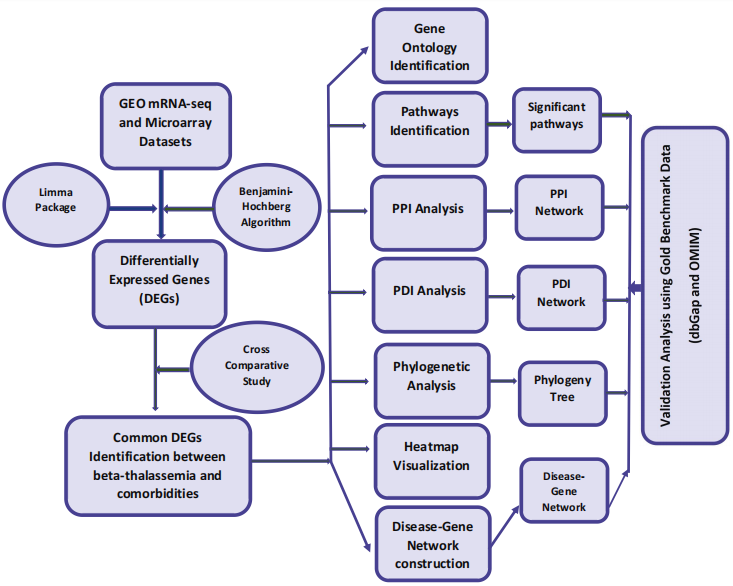
\includegraphics[width=15cm]{./fig/p1.PNG}
\end{center}
\caption{Working flow diagram of this investigation}
\label{fig:dataset_mass_images}
\end{figure}

\section{Dataset Information}
\label{sec:sec3_2}

This study investigated mRNA-seq datasets for BT, PCOS, hypothyroidism, ACM, and arrhythmia, and microarray datasets for T2D and hypogonadism, available in Gene Expression Omnibus (GEO), which is maintained by National Center for Biotechnology Information (NCBI) \cite{b3}, to identify the genetic link between beta-thalassemia and its comorbidities. Each and every datasets has two group normal tissue and malignant or affected tissue. This work compares these normal and malignant samples to indicate which genes are expressed differentially. Those differences can then point out the possible genetic links between BT and its comorbidities.

For BT, GSE117221 GEO mRNA-seq dataset are selected which has total 49 samples. 17 samples are normal tissue that means healthy patient and 32 samples are malignant tissue where (15 samples for thalassemia intermediate and 17 samples for thalassemia major) both type of patients are either female or male. 

For T2D, GSE25724 expression profiling by array genes are selected with 13 samples where 7 samples for type 2 diabetes patients and 6 samples for non-diabetic patients. 
GSE216609 mRNA-seq datasets are selected for PCOS with total 7 samples where 4 sample for control and 3 samples for polycystic ovary syndrome.

With 8 samples GSE176153 GEO mRNA genes are selected for hypothyroidism where 4 samples for healthy patients and 4 samples for malignant patients for both male and female. 
For ACM RNA-seq datasets are selected from NCBI. Its GEO accession is GSE233780 with 12 samples where 6 samples for ACM and other 6 for healthy control. 

GSE26966 GEO microarray datasets are used for hypogonadism with 23 samples where 9 samples for normal pituitary and 14 samples for gonadotrope tumor. 

For arrhythmia GSE175944 mRNA-seq datasets are collected which introduced the most common arrhythmia is atrial fibrillation with 6 samples where 3 samples for control patient and 3 samples for case samples. 

Table 3-1 provides a detailed representation of datasets including GEO accession id, Gender (no. of male and no. of female), samples (divided into case and control groups), associated diseases and source name that indicates the tissue type, cell type or experimental conditions.

% \begin{table}[h]
% \caption{Augmentation Parameters}
% \begin{center}
% \begin{tabular}{|c|c|c|}
% \hline
% \textbf{Augmentation Technique} & \textbf{Parameter} & \textbf{Value} \\
% \hline
% \multirow{4}{*}{RGB Shift} 
% & R Shift & 5 \\ \cline{2-3}
% & G Shift & 5 \\ \cline{2-3}
% & B Shift & 5 \\ \cline{2-3}
% & Probability & 0.7 \\
% \hline
% Random Brightness & Probability & 0.7 \\
% \hline
% \multirow{2}{*}{Motion Blur} 
% & Blur & 7 \\ \cline{2-3} & Probability & 0.7 \\
% \hline
% \end{tabular}
% \caption{Augmentation Parameters}
% \label{tab:augmentation}
% \end{center}
% \end{table}

As a result of these augmentation processes, the dataset was expanded to a total of 7,500 samples, providing greater variety and resilience against overfitting. After performing feature extraction on the augmented dataset, the data was partitioned into two subsets. Following standard machine learning practices, 80\% of the data (6,000 samples) was allocated for training the model, while the remaining 20\% (1,500 samples) was used for testing.

\newpage
\section{Proposed Deep Learning Architectures}
\label{sec:sec3_3}
For BdSL classification, this study used pre-trained convolutional neural networks, ResNet-50 for feature extraction and evaluating two classifiers SVM (Support Vector Machine) and CNN (Convolutional Neural Network) for the final classification job.

\begin{figure}[H]
\begin{center}
    % First row of images
    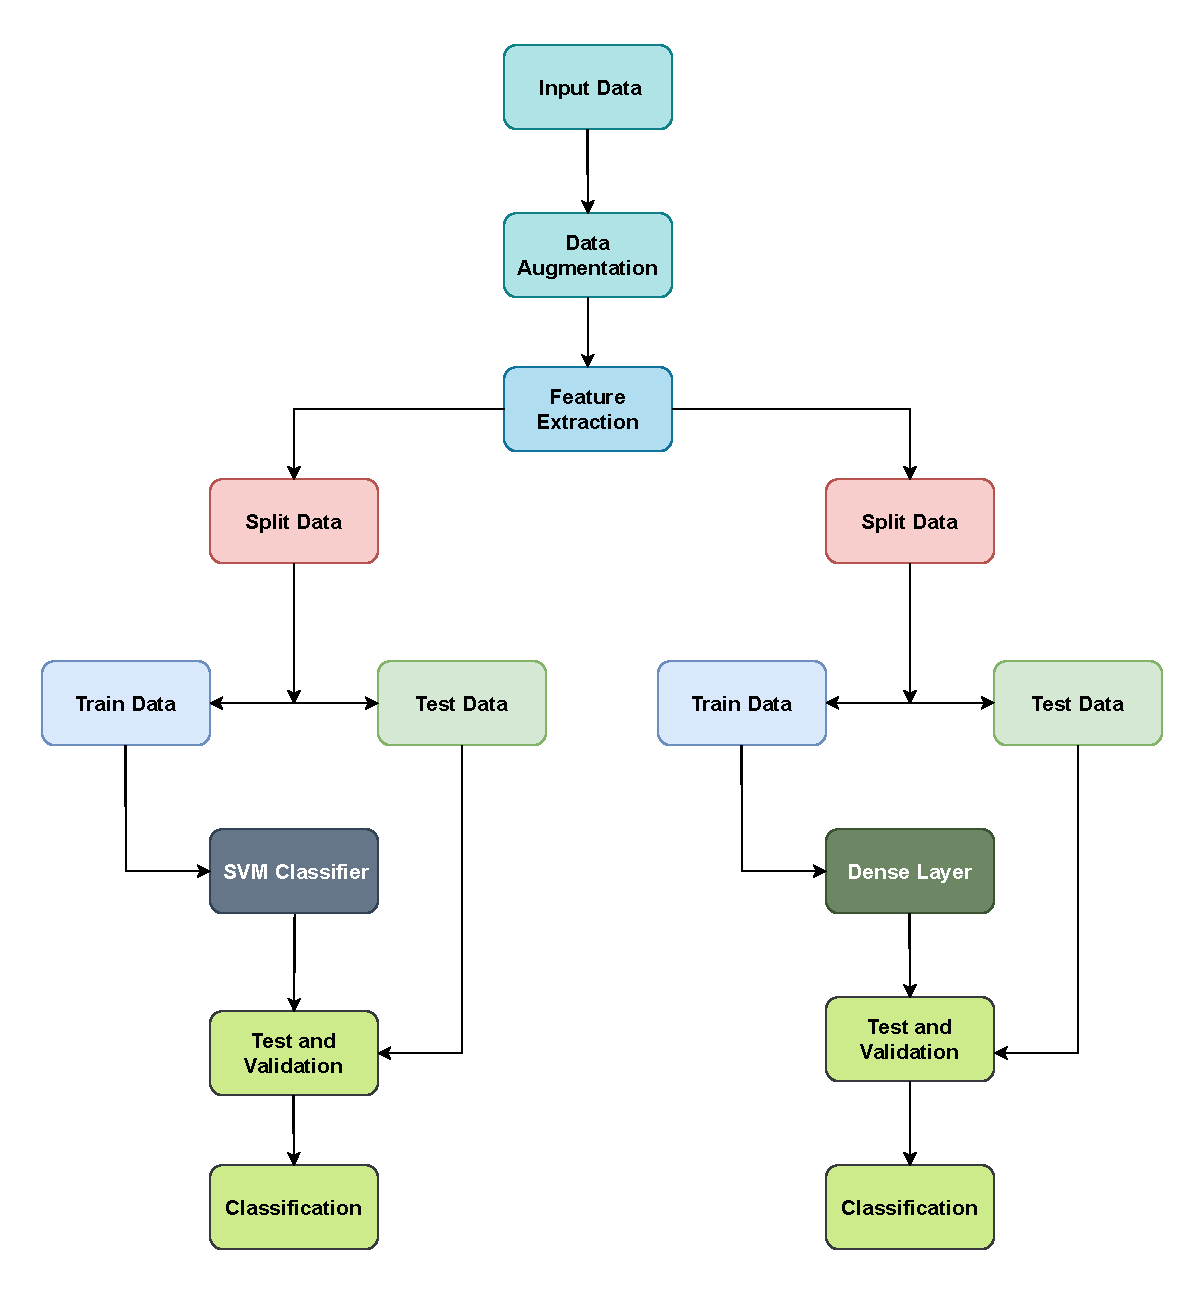
\includegraphics[width=15cm]{./fig/methodology.pdf}
\caption{Procedure of methodological steps.}
\label{tab:augmentation}
\end{center}
\end{figure}

\newpage
\subsection{ResNet-50}
\label{sec:sec3_3_1}
ResNet-50 is a deep convolutional neural network that is 50 layers deep and is part of the Residual Network (ResNet) family \cite{b25}.This architecture allows the network to learn residual mappings, which are easier to optimize compared to traditional raw mappings, enabling deeper networks to achieve higher accuracy. ResNet-50 processes input images of size 224x224x3 (RGB) and outputs feature maps or class probabilities depending on the task. With approximately 25.6 million parameters. ResNet-50 is widely used in computer vision tasks such as image classification, object detection, and feature extraction due to its high accuracy and efficient training.

\begin{figure}[H]
\begin{center}
 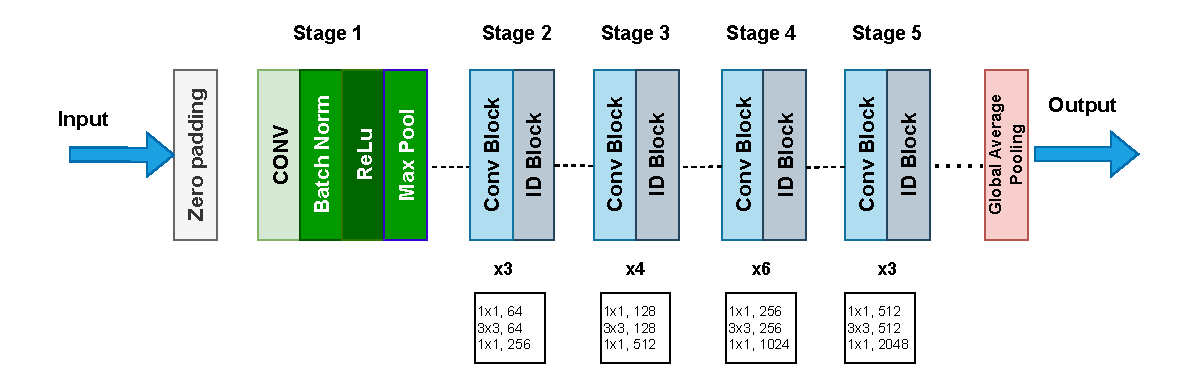
\includegraphics[width=15cm]{./fig/ResNet50.pdf}
\caption{ResNet-50 architecture.}
\label{tab:ResNet-50}
\end{center}
\end{figure}

\subsection{Support Vector Machine (SVM)}
\label{sec:sec3_3_2}
The Support Vector Machine (SVM) is a supervised machine learning technique extensively employed for classification and regression tasks. It is very productive for high-dimensional data and limited datasets. Support Vector Machines (SVM) seek to identify the ideal hyperplane that maximises the margin between classes, hence assuring effective generalisation to novel data. For linearly separable data, SVM employs a linear hyperplane; conversely, for non-linear data, it applies kernel functions to map the data into a higher-dimensional space for efficient separation.

\subsection{Dense Layer}
\label{sec:sec3_3_3}
A custom neural network was designed using TensorFlow's Keras API for multi-class classification. The architecture comprises an input layer followed by two fully connected layers with 256 and 128 neurons, respectively, each using the ReLU activation function to introduce non-linearity. Dropout layers with a 30\% rate were added after each dense layer to mitigate overfitting by randomly deactivating neurons during training. The output layer uses a softmax activation function to generate class probabilities. The model was compiled using the Adam optimizer, which adjusts learning rates dynamically, and sparse categorical cross-entropy as the loss function:
\[
L = -\sum_{i=1}^{n} \log(\hat{y}_i, y_i),
\]

where \(\hat{y}_i, y_i\) represent the predicted probability and the true class, respectively.

\begin{table}[H]
  \begin{tabular}{|p{2.7cm}|p{2.3cm}|p{3cm}|p{1.8cm}|p{1.8cm}|p{1cm}|p{1cm}|}
     \hline
     \textbf{Model Name}&\textbf{Optimization Algorithm}&\textbf{Loss\newline Function}&\textbf{Activation\newline Function\newline in Hidden \newline Layer}&\textbf{Activation\newline Function\newline in Output \newline Layer}&\textbf{Batch\newline Size}&\textbf{Epoch}\\
    \hline
    \textbf{ResNet-50} & Adam & Sparse categorical cross entropy & ReLu & Softmax & 32 & 100\\
    \hline
    \end{tabular}
    \caption{Parameter Used in Dense Layer classification.}
    \label{tab:hyperparameter}
\end{table}